% !TEX root = MSTAT19.tex
% This work is licensed under the Creative Commons
% Attribution-NonCommercial-ShareAlike 4.0 International License. To view a copy
% of this license, visit http://creativecommons.org/licenses/by-nc-sa/4.0/ or
% send a letter to Creative Commons, PO Box 1866, Mountain View, CA 94042, USA.

\section{Verteilungskonvergenz im Raum stetiger Funktionen} %7
Sei $I:=\intervall ab$ mit $a < b$ und
\begin{align*}
	C:=C(I):=\set[\big]{ f:I⟶ℝ\mid f\text{ stetig}}
\end{align*}
versehen mit der Supremumsmetrik
\begin{align*}
	d(f,g)& := \sup_{t∈ I} \abs{f(t)-g(t)} \qquad ∀ f, g∈ C.
\end{align*}
Gemäß Beispiel \ref{beisp2.6} ist $(C,d)$ separabel.
Die Borel-$σ$-Algebra
$\B(C):=\B_d\argu[\big]{C(I)}$,
die durch $d$ induziert wird,
gestattet eine einfache Beschreibung.
Dazu:

\begin{definition}\ %7.1
	\begin{enumerate}[label=(\arabic*)]
		\item Sei $t∈ I$. Die Abbildung
		\begin{align*}
			π_t:C⟶ℝ,\qquadπ_t(f):=f(t)\qquad∀ f∈ C
		\end{align*}
		heißt \define{Projektion in $t$}.
		\item Sei $T:=\set[\big]{ t_1,…,t_k}⊆ I,k∈ℕ$. Die Abbildung
		\begin{align*}
			π_T:C⟶ℝ^k,\qquad π_T(f):=\klammern[\big]{f(t_1),…,f(t_k)}=:
			\klammern[\big]{f(t)}_{t∈ T}\qquad∀ f∈ C
		\end{align*}
		heißt \define{Projektion in $T$}.
	\end{enumerate}
\end{definition}

\begin{satz}\label{satz7.2}
	\begin{align*}
		\B(C)
		=σ\argu[\big]{π_t:t∈ I}=σ\klammern[\big]{π_T:T⊆ I,T\text{ endlich}}
		% =σ\argu{\set[\big]{ π_t^{-1}(B):t∈ I,B∈\B(ℝ)}}
		% erklärt in nächster Erinnerung
	\end{align*}
	Das heißt, die Borel-$σ$-Algebra ist die \enquote{kleinste $σ$-Algebra, sodass alle $π_t$ messbar sind}.
\end{satz}

\begin{erinnerung}
	\begin{align*}
		σ\argu[\big]{π_t:t∈ I}
		\overset{\Def}&{=}
		σ\argu{\set[\big]{ π_t^{-1}(B):t∈ I,B∈\B(ℝ)}}\\
		σ \argu{π_T:T⊆ I,T\text{ endlich}}
		\overset{\Def}&{=}
		σ\argu{\set[\big]{π_T^{-1}(B):T⊆ I\text{ endlich, }B∈\B(ℝ)}}\\
		σ\colon\Potenzmenge{\Potenzmenge{Ω}} &⟶ \Potenzmenge{\Potenzmenge{Ω}},\\
		σ(\mathcal{M})&:=\bigcap_{\begin{subarray}{c}
			\A⊆\Potenzmenge{Ω}~σ\text{-Algebra}\\
			\mathcal{M}⊆\A
		\end{subarray}}
		\A
	\end{align*}
\end{erinnerung}

\begin{proof}
	Da $π_t=π_{\set{t}}$ und mit $T=\set {t}$, folgt
	\begin{align}\label{eqProof7.2(1)}\tag{1}
		σ\argu[\Big]{π_t:t∈ I}
		⊆σ \argu{π_T:T⊆ I\text{ endlich}}
	\end{align}
	Weiterhin gilt:
	\begin{align*}
		&\norm[\big]{π_T(f)-π_T(g)}_∞
		=\max_{1≤ i≤ k} \abs{f(t_i)-g(t_i)}
		≤ d(f,g)\qquad∀ f,g∈ C,∀\, T=\set{ t_1,…,t_k}⊆ I\\
		&⇒π_T:(C,d)⟶ℝ^d\text{ ist stetig}
	\end{align*}
	Aus Lemma \ref{Lemma3.2} \ref{it:3.2StetigMessbar} folgt,
	dass $π_T \colon \B(C) ⟶ \B(ℝ^k)$ messbar ist für alle endlichen Teilmengen $T ⊆ I$.
	Da $σ\argu{π_T:T⊆ I\text{ endlich}}$ die \emph{kleinste} $σ$-Algebra auf $C$ ist, bzgl.\ der \emph{alle} $π_T,T⊆ I$ endlich, messbar sind, folgt
	\begin{align}\label{eqProof7.2(2)}\tag{2}
		σ\argu[\big]{π_T:T⊆ I,T\text{ endlich}} ⊆ \B(C)
	\end{align}
	Wegen \eqref{eqProof7.2(1)} und \eqref{eqProof7.2(2)} bleibt zu zeigen:
	\begin{align}\label{eqProof7.2(3)}\tag{3}
		\B(C) ⊆ σ\argu[\Big]{π_t:t∈ I} =: \tilde B
	\end{align}
	Dazu sei $G∈\G(C)$, d.\,h.\ $G⊆ C$ offen.
	Gemäß Satz \ref{satz2.9} existieren $f_i∈ C$, $ε_i>0$, $i∈ℕ$ mit
	\begin{align}\label{eqProof7.2(4)}\tag{4}
		G = \Union_{i∈ℕ} B \argu[\big]{f_i,ε_i} \quad \text{(abzählbare Vereinigung offener Kugeln)}.
	\end{align}
	Für jede offene Kugel
	\begin{align}\label{eqProof7.2(5)}\tag{5}
		B(f,ε)
		&=\set[\big]{ g∈ C:d(g,f)<ε}
		=\Union_{k∈ℕ}\underbrace{\set{ g∈ C:d(g,f)≤ε-\frac{1}{k}}}_{=\text{ abgeschlossene Kugel}}
	\end{align}
	Betrachte daher eine beliebige \emph{abgeschlosssene} Kugel
	\begin{align*}
		\abschluss{B}(f,δ)
		% CHECKED: '\abschluss' used.
		&=\set[\Big]{ g ∈ C : \sup_{t∈ I} \abs[\big]{g(t)-f(t)} ≤ δ}\\
		&=\set[\Big]{ g ∈ C : \sup_{t∈ I∩ℚ} \abs[\big]{g(t)-f(t)} ≤ δ}\\
		&=\bigcap_{t∈ I ∩ ℚ}\set[\Big]{ g ∈ C : \abs[\big]{g(t)-f(t)} ≤ δ}\\
		&=\bigcap_{t∈ I ∩ ℚ} \underbrace{\set[\Big]{ g ∈ C : f(t) - δ
		≤ \overbrace{g(t)}^{=π_t(g)}
		≤ f(t) + δ}}_{π_t^{-1} \klammern[\Big]{\eckigeKlammern[\big]{f(t)-δ,f(t)+δ}} ∈ \tilde{\B}}\\
		&⇒
		\overline{B}(f,δ) ∈ \tilde{\B} \qquad ∀ f ∈ C \, ∀ δ > 0\\
		&\overset{\eqref{eqProof7.2(5)}}{⇒}
		B(f,ε)∈\tilde{\B}\qquad∀ f∈ C \, ∀ε>0\\
		&\overset{\eqref{eqProof7.2(4)}}{⇒}
		G∈\tilde{\B}\\
		&⇒
		\G(C)⊆\tilde{\B}\\
		&⇒σ\argu[\big]{\G(C)}=\B(C)⊆\tilde{\B}
		\qedhere
	\end{align*}
\end{proof}
%Ferger hat Borel-Mengen am Anfang des Studiums gehasst, weil er sie nicht verstanden hat. Jetzt sieht er das anders.
% Auch mit inf und sup konnte er sich lange nicht anfreunden. Jetzt hat er eine Gruppe
% von Erstis, die er motivieren soll als Mentor, denen er die Definition des inf aufschreibt
% und sie motiviert sich mit dem inf anzufreunden.

\begin{defi}
	Ein stochastischer Prozess $\set[\big]{ X(t):t∈ I}$ heißt \define{indiziert nach $I$ (über $(Ω,\A)$)}
		\begin{align*}
	:⇔ X(t):(Ω,\A)⟶(ℝ,\B(ℝ)),
	\qquad ω↦ X(t)(ω) = X(t, ω) \quad
		\text{ist messbar } ∀ t ∈ I
	\end{align*}
	%Ferger: "Trage ich zu einer Verwirrung bei?"
	Schreibweise: $X(t,ω):=X(t)(ω)$

	Falls die \define{Pfade/ Trajektorien}
	\begin{align*}
		X(·,ω) \colon I ⟶ ℝ, \qquad t↦ X(t,ω) \qquad (ω ∈ Ω)
	\end{align*}
	stetig sind (für alle $ω∈Ω$), so liefert die Zuordnung $ω↦ X(·,ω)$ eine Abbildung $X:Ω⟶ C(I)$.
	Diese Abbildung $X$ heißt \define{Pfadabbildung} des stochastischen Prozesses und wird mit diesem identifiziert, genauer:

	Für einen stochastischen Prozess $X\colon I×Ω⟶ℝ$ gilt:
	\begin{itemize}
		\item $X\colon I⟶ℝ,\qquad t↦ X(t,ω)$ heißt \define{Pfad} für jedes $ω∈Ω$
		\item $X\colonΩ⟶ℝ,\qquadω↦ X(t,ω)$ ist eine einzelne ZV für jedes $t∈ I$
		\item $X\colonΩ⟶ (I⟶ℝ),\qquad ω↦(t↦ X(t,ω))$ heißt \define{Pfadabbildung}
		\item Falls alle Pfade stetig (also $X$ ein \define{stetiger stochastischer Prozess} ist) sind, gilt $I⟶ℝ=C(I)$.
		\item Man kann einen (stetigen) stochastischen Prozess mit seiner Pfadabbildung identifizieren:
		\begin{align}\label{eqIdentifiereSP}
			\set[\big]{ X(t)\mid t∈ I, X(t)\colonΩ⟶ℝ}
			\cong X\colonΩ⟶ C(I)
		\end{align}
	\end{itemize}
\end{defi}

Satz \ref{satz7.2} liefert ein sehr handliches Kriterium für die Messbarkeit von allgemeinen Abbildungen $X \colon Ω ⟶ C$.

\begin{satz}\label{satz7.3}
	Sei $(Ω,\A)$ messbarer Raum und $C:=C(I)$ versehen mit der Borel-$σ$-Algebra $\B(C)$ sowie $X \colon Ω ⟶ C$. Dann gilt:
	\begin{align*}
		X\text{ ist } \A\text{-}\B(C)\text{-messbar}⇔∀ t∈ I:π_t∘ X\text { ist }\A\text{-}\B(ℝ)\text{-messbar}
	\end{align*}
\end{satz}

\begin{proof}
	Erinnere an das \undefine{Messbarkeitslemma}:
	\begin{lem}[{Messbarkeitslemma, vgl.\ \cite[Satz 1.2.11]{gaensslerstute1977Wahrscheinlichkeitstheorie}}] % lem = lemma without number
		Sei $(Ω,\A)$ messbarer Raum, $Ω\neq∅$, $(f_t)_{t∈ T}$ eine Familie von Abbildungen
		$f_t \colon Ω ⟶ (Ω_t, \A_t)$ wobei $(Ω_t,\A_t)$ messbarer Raum für alle $t∈ T$,
		$T\neq∅$ beliebige Indexmenge.
		Ferner sei
		\begin{align*}
			\A':=σ\argu[\big]{f_t:t∈ T}\stackeq{\text{Def}}σ\klammern{\Union_{t∈ T} f_t^{-1}(\A_t)}
		\end{align*}
		Dann gilt für eine Abbildung $Z:Ω⟶Ω'$:
		\begin{align*}
			Z\text{ ist }\A\text{-}\A'\text{-messbar}⇔∀ t∈ T: f_t∘ Z\text{ ist }\A\text{-}\A_t\text{-messbar}
		\end{align*}
	\end{lem} % end lemma Messbarkeitslemma
	Im Falle von Satz \ref{satz7.3}: $Ω'=C$,
	$\A' = σ\argu[\big]{π_t : t ∈ I} \stackeq{\ref{satz7.2}}\B(C)$,
	$f_t=π_t$, $Ω_t = ℝ$, $\A_t = \B(ℝ)$, $T=I$,
	$Z=X$.
\end{proof}

Stochastische Prozesse mit stetigen Pfaden nennt man \define{stetige} stochastische Prozesse.
Satz \ref{satz7.3} besagt nun:
Die Pfadabbildung eines jeden stetigen stochastischen Prozesses ist $\A\text{-}\B(C)$-messbar.
Insbesondere folgt:
\emph{Jeder stetige stochastische Prozess indiziert nach $I$ kann aufgefasst werden als Zufallsvariable im metrischen Raum $\klammern[\big]{C(I),d}$.}

\begin{beispiel}\label{beispiel7.4}
	Sei $(ξ_i)_{i∈ℕ}$ % = (ξ_i(ω))_{i ∈ ℕ}$
	eine Folge von reellen Zufallsvariablen über $(Ω,\A)$ und für $n∈ℕ$ sei
	\begin{align*}
		S_k:=\sum_{i=1}^k ξ_i\qquad∀0≤ k≤ n\qquad S_0:=0
	\end{align*}
	Der Polygonzug $X_n$ durch die Punkte $\klammern{\frac{k}{n},\frac{1}{√{n}} S_k}, 0 ≤ k ≤ n$ heißt \define{$n$-ter Partialsummenprozess}.
	\begin{figure}[H]
		\begin{center}
			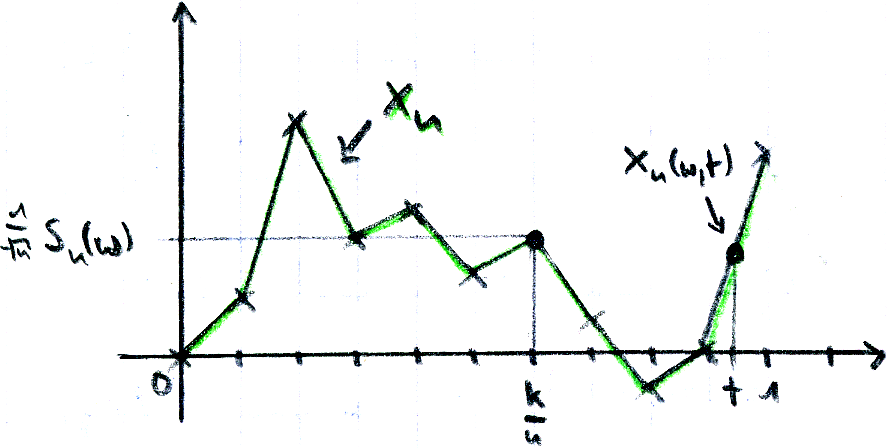
\includegraphics[width=1\textwidth]{./pics/MSTAT001.png}
			\caption{Partialsummenprozess mit $n=10$, $k=6$}
			\label{AbbPartialsummenprozess}
		\end{center}
	\end{figure}
	Mit der Zwei-Punkte-Formel der Geradengleichung folgt:
	\begin{align*}
		X_n(t)
		= \frac{1}{√{n}} \sum_{i=1}^{\floor{nt}} ξ_i + \frac{1}{√{n}} \klammern[\big]{nt-\floor{nt}} · ξ_{\floor{nt} + 1} \qquad ∀ t ∈ \intervall01 = I
	\end{align*}
	Hierbei ist die Gaußklammer (Abrundefunktion) wie folgt definiert:
	\begin{align*}
		\floor u := [u] := \max\set[\big]{l∈\Z : l≤ n}
	\end{align*}
	$X_n(t)$ ist eine reelle Zufallsvariable für alle $t∈ I$.
	Gemäß Konstruktion (Polygonzug) ist jeder Pfad von $X_n$ stetig auf $[0,1]$.
	Aus Satz \ref{satz7.3} folgt, dass $X_n~\A\text{-}\B(C)$-messbar ist, also Zufallsvariable in $\klammern[\Big]{C\klammern[\big]{[0,1]},d}$.

	Weitere Anwendung von Satz \ref{satz7.2}:
\end{beispiel}

\begin{satz}\label{satz7.5}
	\begin{enumerate}[label=(\arabic*)]
		\item \label{it:7.5Masse} $P,Q$ seien Wahrscheinlichkeitsmaße auf $\klammern{C, \B(C)}$. Dann gilt:
			\begin{align*}
				P=Q⇔∀ T⊆ I\text{ endlich}: P∘π_T^{-1}=Q∘π_T^{-1}
			\end{align*}
		\item \label{it:7.5Vars} $X,Y$ seien Zufallsvariablen in $\klammern[\big]{C(I),d}$. Dann gilt:
			\begin{align*}
				X\stackeq{\L}Y⇔∀ T⊆ I\text{ endlich }: π_T(X)\stackeq{\L}π_T(Y)
			\end{align*}
	\end{enumerate}
\end{satz}

\begin{proof}~
	\paragraph{Zu \ref{it:7.5Masse}, zeige \enquote{$⇒$}} Trivial.
	\paragraph{Zu \ref{it:7.5Masse}, zeige \enquote{$⇐$}}
	Gemäß Satz \ref{satz7.2} ist
	\begin{align*}
		\mathcal{E}:=\set{π_T^{-1}(A):A∈\B\argu{ℝ^{\measure{T}}},T⊆ I\text{ endlich}}
	\end{align*}
	ein Erzeuger von $\B(C)$, d.\,h.\ $\B(C)=σ(\mathcal{E})$. Erinnerung:
	\begin{align*}
		g^{-1}(\mathcal{C})&:=\set[\big]{ g^{-1}(C):C∈\mathcal{C}}\text{ für Mengenfamilie }\mathcal{C}\\
		\B(C)&\stackeq{\ref{satz7.2}}σ\argu[\big]{π_T:T⊆ I\text{ endlich}}
		=σ\argu[\Bigg]{\underbrace{
			\Union_{
				\begin{subarray}{c}
					T⊆ I \\
					T\text{ endlich}
				\end{subarray}}
				π_T^{-1} \argu{ \B\argu{ℝ^{\abs{T}}}}
		}_{=\mathcal{E}}}
	\end{align*}
	Nach Voraussetzung gilt:
	\begin{align*}
		P \argu{π_T^{-1}(A)} \overset{\text{Def}}= P∘π_T^{-1}(A)
		&= Q∘π_T^{-1}(A) = Q \argu{π_T^{-1}(A)} \qquad ∀ A ∈ \B \klammern{ℝ^{\abs{T}}}\\
		⇒
		\restr{P}{\mathcal{E}} &= \restr{Q}{\mathcal{E}}
	\end{align*}
	$\mathcal{E}$ ist durchschnittsstabil (nachrechnen!).
	Damit liefert der \undefine{Maßeindeutigkeitssatz}, dass $P=Q$ auf $σ(\mathcal{E})=\B(C)$.
	(Der Maßeindeutigkeitssatz besagt:
	zwei Wahrscheinlichkeitsmaße, die auf einen schnittstabilen Mengensystem überein stimmen, stimmen auch auf dessen Erzeugnis überein.)
	\paragraph{Zeige \ref{it:7.5Vars}}
	\begin{align*}
		X\stackeq{\L} Y
		\overset{\text{Def}}&{⇔}
		\P∘ X^{-1}=\P∘ Y^{-1}\\
		\overset{\ref{it:7.5Masse}}&{⇔}
		\underbrace{\argu{\P∘ X^{-1}}∘ π_T^{-1}}_{=\P∘\klammern{π_T∘ X}^{-1}}
		=\underbrace{\klammern{\P∘ Y^{-1}}∘π_T^{-1}}_{=\P∘\klammern{π_T∘ Y}^{-1}}
		&∀ T⊆ I\text{ endlich}\\
		&⇔
		\underbrace{π_T∘ X}_{=π_T(X)}\stackeq{\L}\underbrace{π_T∘ Y}_{=π_T(Y)}
		&∀ T⊆ I\text{ endlich}
		& \qedhere
	\end{align*}
\end{proof}

\begin{bemerkungnr} %7.6
	Die Wahrscheinlichkeitsmaße $\P∘\klammern[\big]{π_T∘ X}^{-1}$ bzw.\ die Verteilungen
	% CHECKED: 'bzw.' used.
	\begin{align*}
		π_T(X) &= \klammern[\big]{X(t_1), …, X(t_k)} & ∀ & T =\set{t_1,…,t_k} ⊆ I\text{, genauer:}\\
		π_T\argu[\big]{X(ω)} &= \klammern{X(ω)(t_1),…,X(ω)(t_k)} & ∀ & ω∈Ω, ∀ T = \set{ t_1,…,t_k}⊆ I\\
		&π_T∘ X\colonΩ⟶ C⟶ℝ_k
	\end{align*}
	heißen \define{endlich dimensionale Randverteilungen von $\P$} bzw.\ \define{von $X$}.
	% CHECKED: 'bzw.' used.
	Insbesondere ist gemäß \ref{satz7.5} \ref{it:7.5Vars} die Verteilung eines stetigen stochastischen Prozesses $X$ aufgefasst als Zufallsvariable in $C$ eindeutig durch die Verteilungen der Vektoren
	\begin{align*}
		\klammern[\big]{X(t_1),…,X(t_k)},\qquad t_1,…,t_k∈ I,k∈ℕ
	\end{align*}
	festgelegt.
\end{bemerkungnr}

